\documentclass[aspectratio=1610, english]{beamer} 
\usepackage{babel}
\makeatletter
\@ifclasswith{beamer}{polish}{
	\usepackage{polski}
}

\graphicspath{{static/}} 
\makeatother
\usepackage[utf8x]{inputenc}

\mode<beamer>{ 	% In the 'beamer' mode
	\hypersetup{pdfpagemode=FullScreen}         % Enable Full screen mode
	\usetheme[parttitle=rightfooter]{AGH}       % Show part title in right footer
	%\usetheme[nosidebar]{AGH}                  % Do not show sidebar on non-title slides
	%\usetheme[nosidebar, margins=1em]{AGH}     % Do not show sidebar on non-title slides and set both margins (left / right) to 1em
}
\mode<handout>{	% In the 'handout' mode
	\hypersetup{pdfpagemode=None}		
	\usepackage{pgfpages}
	\pgfpagesuselayout{4 on 1}[a4paper,border shrink=5mm,landscape]	% Show 4 slides on 1 page
	\pgfpageslogicalpageoptions{1}{border code=\pgfusepath{stroke}}
	\pgfpageslogicalpageoptions{2}{border code=\pgfusepath{stroke}}
	\pgfpageslogicalpageoptions{3}{border code=\pgfusepath{stroke}}
	\pgfpageslogicalpageoptions{4}{border code=\pgfusepath{stroke}}
  	\usetheme{boxes}
  	\addheadbox{structure}{\quad\insertpart\hfill\insertsection\hfill\insertsubsection\qquad}          % Content of header
 	\addfootbox{structure}{\quad\insertshortauthor\hfill\insertframenumber\hfill\insertsubtitle\qquad} % Content of footer
}

\AtBeginPart{ % At begin part: display its name
	\frame{\partpage}
} 
\author[Aleksandra Poreba]{Aleksandra Poreba}
\date{}

	\title{HZZ Analysis}
	\subtitle{Introduction to the Particle Physics Data Analysis}

%%%%%%%%%%%%%%%%%
\begin{document}
\maketitle

%%%%%%%%%%%%%%%%
\begin{frame}{Outline}
	\tableofcontents
\end{frame}

%%%%%%%%%%%%%%%%%%%%%%%
\section{Physics motivation}

\begin{frame}
\frametitle{Physics motivation}
The physics motivation for the measurement:
\begin{itemize}
\item a good test for the SM,
\item a measurement of inclusive and differential fiducial cross sections,
\item
\end{itemize}

\end{frame}

\begin{frame}
\frametitle{The Feynman diagram}

\begin{figure} [H]
\centering
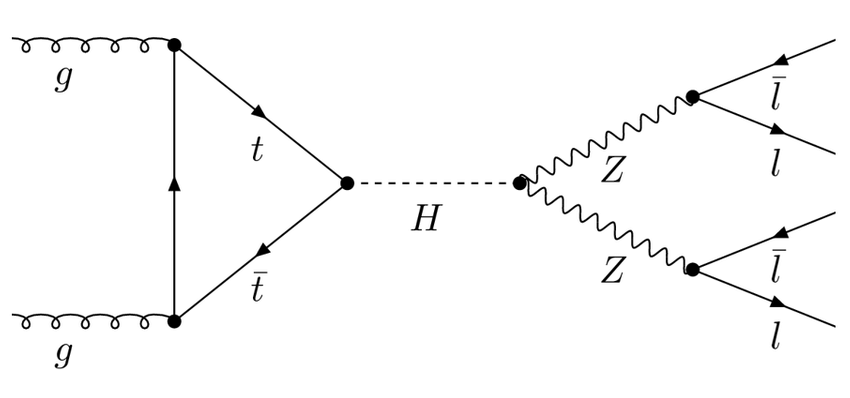
\includegraphics[width=8cm]{feynman_diagram.png}
\caption{Feynman diagram for H→ZZ∗→4ℓ decay \cite{diagram}. }
\end{figure}

\end{frame}

%%%%%%%%%%%%%%%%%%%%%%%
\section{Expected number of events}

\begin{frame}
\frametitle{Expected number of events}


\end{frame}

%%%%%%%%%%%%%%%%%%%%%%%
\section{Event selection}

%%%%%%%%%%%%%%%%%%%%%%%
\section{Background contributions}

%%%%%%%%%%%%%%%%%%%%%%%
\section{Control plots}

\begin{frame}
\frametitle{Number of Leptons}

\begin{figure} [H]
\centering
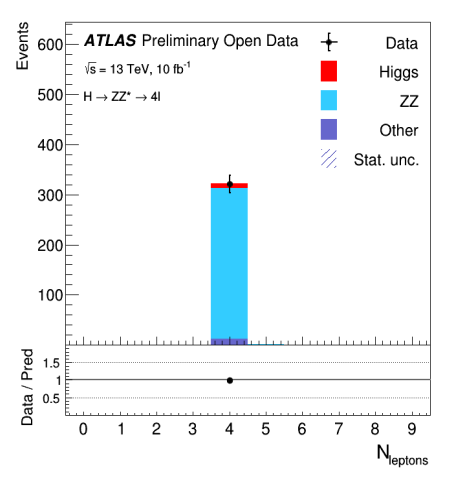
\includegraphics[width=6cm]{hist_n_lept.png}
\caption{The histogram with number of leptons. }
\end{figure}

\end{frame}

%%%%%%%%%%%%%%%%%%%%%%%
\section{Ideas for possible measurements}

%%%%%%%%%%%%%%%%%%%%%%%
\section{Bibliography}
%%%%%%%%%%%%%%%%%%%%%%%
\begin{frame}[allowframebreaks]{Bibliography}
	\begin{thebibliography}{9}
		\setbeamertemplate{bibliography item}[article]
		\bibitem{opendata}
			{The ATLAS collaboration\newblock Review of the 13 TeV ATLAS Open Data release \newblock \url{https://cds.cern.ch/record/2707171}}
		\bibitem{hzz}
			{Aaboud, Morad and others \newblock Measurement of inclusive and differential cross sections in the H→ZZ∗→4ℓ decay channel in pp collisions at s√ = 13 TeV with the ATLAS detector \newblock \url{http://dx.doi.org/10.1007/JHEP10(2017)132}}
		\bibitem{diagram}
			{Passon, Oliver \newblock On the interpretation of Feynman diagrams, or, did the LHC experiments observe the Higgs to gamma gamma decay?}
	\end{thebibliography}
\end{frame}
\end{document}
